
\pagebreak

\subsection{Milky Way Scan}

\subsubsection{Observation time}
From our observation spot in Bern, we had to plan the observation time to get the best possible overview of the Milky Way with a wide range in the galactic longitude. In October, when we did this measurments, the maximum elevation of the galactic center is around 13° (in south) at 18:30 MESZ. However, limitations in the field of view of the SRT had to be considered to choose the best observation time:

\begin{itemize}
    \item At 18:30 MESZ, the galactic center ($l_g=\SI{0}{\degree}$) could be included in the scan but at galactic longitudes of $l_g>\SI{120}{\degree}$, the SRT run in the lower azimuth limit from EXWI building at around 40° (north east).
    \item At later times, the galactic center is already descending and but the higher galactic longitudes are moving inside visible area of the SRT.
    \item At 22:00 MESZ, the galactic center is at the horizon and no more visible but the galactic plane is almost perpendicular to the horizontal plane and it is in the visible area of the SRT up to galactic longitude $l_g=\SI{180}{\degree}$. Only limitation is the main building of the University Bern, that covers the view partially. We decided to do the scan at this time. 
\end{itemize}
    
The scan path is illustrated in figure \ref{fig:mw_scan_stellarium}. We chose the scan path start at galactic longitude of 10° and end at 170° to avoid lower elevations than 10° as the noise level of the ground thermal radiation is dominating there.


\begin{figure}[H]
    \centering
    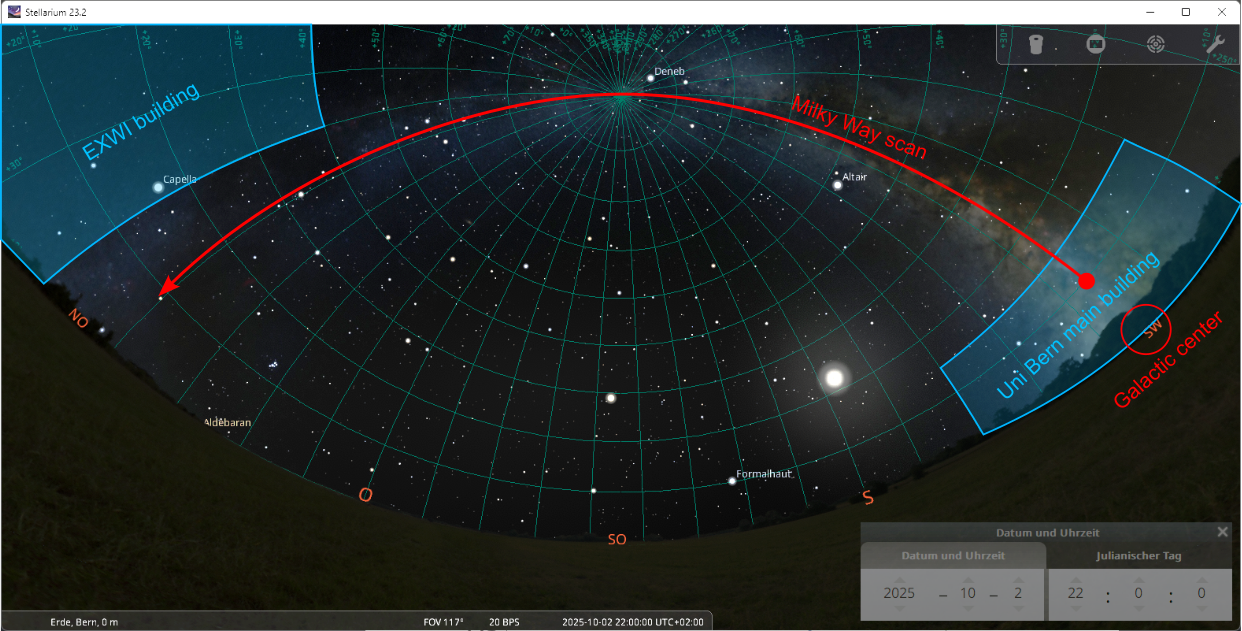
\includegraphics[width=12cm]{assets/stellariumView_edit.png}
    \caption{View of the Milky Way scan in Stellarium [XXX] with SRT field of view limitations (blue).}
    \label{fig:mw_scan_stellarium}
\end{figure}

\subsubsection{Measurement}
It was hard to find out, how to correctly set up the Lab View tool for a Milky Way scan, as the angular range input fields belong to azimuthal coordinates rather than galactic. Finally we found, that the tool uses wrong (mirrored) galactic coordinates (correct longitude is $l_g=\SI{360}{\degree}-l_{srt}$ to enter in the azimuth fields. We chose a step size of $\Delta l_g=\SI{0.25}{\degree}$ with 1000 ms integration time what resulted in a measurement time of 28 min to scan from 10° to 170° in galactic coordinates. Figure \ref{fig:mw_scan_polar} shows the scan path in a polar diagram:

\begin{figure}[H]
    \centering
    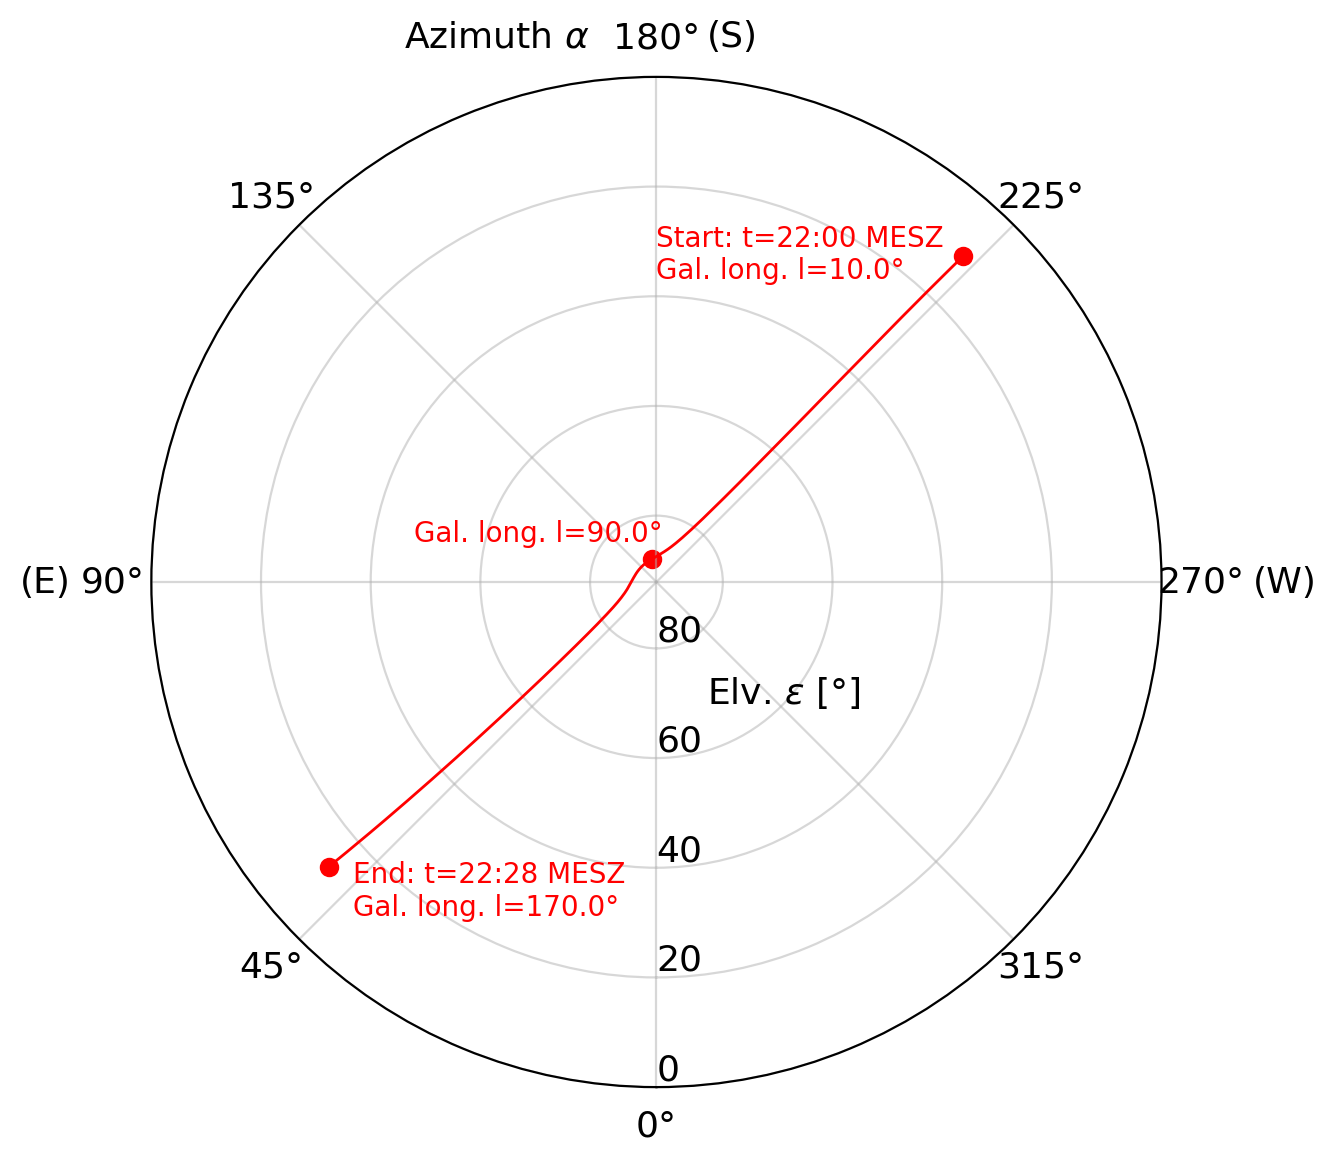
\includegraphics[width=10cm]{assets/mw_scan_polar.png}
    \caption{Polar plot of the Milky Way scan}
    \label{fig:mw_scan_polar}
\end{figure}

Figure \ref{fig:mw_spectrum_plot} shows the received power spectrum of the Milky Way scan. Vertically centred is the carrier frequency $f_c$ of the spectrometer, that matches the 21 cm wavelength of neutral oxygen ($f_c=$\SI{1420.4}{\giga\hertz}).
The brighter regions where more power was received show the emission from the hydrogen clouds in the Milky Way disc. A positive relative velocity $v_r>0$ between the earth and the emitting cloud result in a red shift and the maximal power received is shown in the lower half of the plot. For $v_r<0$ it is blue-shifted in the upper half. Some interesting regions are marked in red and will be discussed later.


\begin{figure}[H]
    \centering
    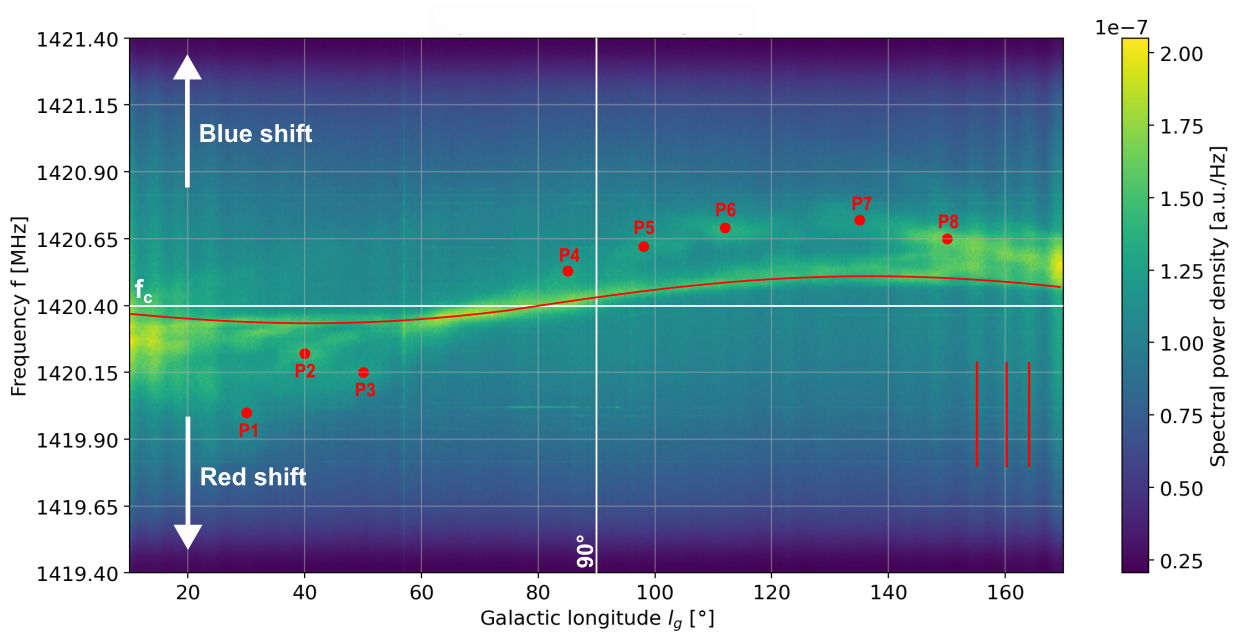
\includegraphics[width=\textwidth]{assets/spectrum_plot_edit.png}
    \caption{Received spectral power density vs. galactic longitude @ at zero latitude (galactic plane)}
    \label{fig:mw_spectrum_plot}
\end{figure}

We can identify following features in the spectrum plot:

\begin{itemize}
    \item The received spectrum from the hydrogen clouds is clearly red-shifted at longitudes below ~70° and blue shifted above. This was expected according explanation in section XXXXXX.
    \item The highest power density received, follow a sine shaped trend line (marked red). Most likely, this is the emission from the Perseus spiral arm of the Milky Way (Refer section \ref{sec:HotSpots}).
    \item There are some interesting regions with high radiation visible. Some of them are marked with Points P1 to P8 and will be discussed in section XXXXXX.
    \item We see some vertical lines of higher power density at low elevations (some marked red). These are caused from the high ground radiation that is amplified in the side lobes of the antenna characteristic as explained in section YYYYYY.
\end{itemize}



\subsubsection{Additional Exercise: Source determination of the hot spots}\label{sec:HotSpots}
In the Milky Way scan plot (figure \ref{fig:mw_spectrum_plot}) we have marked some hot spots of higher radiation. We tried to determine the sources of these spots in the Milky Way galactic disc. We have marked just spots with high red-/blue-shifts since a low shift results in very high inaccuracy in further calculations. \\
 \\
As explained in section ZZZZZ, we get the relation from the relative velocity $v_r$ to the radius $R$ of a radiating object in the galaxy plane in function of the galactic longitude $l_g$ using equation (XXXXXX). We considered the radial velocity as constant $v = v_0$ for all radii $R > 3kpc$, what is true for our positions we discuss. We can transform equation (XXXXX) to get the radius (in units of distance sun$\leftrightarrow$galactic center $R_0$) in function of the relative velocity and the galactic longitude as:

\begin{equation}
	\frac{R}{R_0}=\frac{v_0\cdot sin(l_g)}{v_0\cdot sin(l_g)-v_r}
\end{equation}

We can directly get $v_r$ from the Doppler shift. As $v_r$ is positive for red-shift, it is calculated as:

\begin{equation}
	v_r = \frac{f_c-f}{f_c} c
\end{equation}

From the hot spots marked in figure \ref{fig:mw_spectrum_plot}, we calculated the radii where the radiating source must be located. Finally, the position of the source is the intersection of the circle with the viewing line from the sun along the corresponding galactic longitude. We solved this problem graphically and drew the solution directly into the view of the Milky Way. In case of two solutions, we just marked the one closer to the sun. We did no error considerations for this task but we expect large uncertainties for the positions. Especially the red-shift caused by the orbital velocity of the earth around the sun (what is up to 30 km/s) is not considered and might result in a larger error. For the radii for P1...P8 in figure \ref{fig:mw_spectrum_plot}, we got...

\begin{table}[H]
\centering \footnotesize
\begin{tabular}{| l || r | r || r | r |}
    \hline 
    Point & $l_g$ & $f$ [MHz] & $v_r$ [km/s] & $R/R_0$\\
    \hline
    \hline 
    P1    &  30°  & 1420.00   &  84          & 0.57 \\
    P2    &  40°  & 1420.22   &  38          & 0.79 \\
    P3    &  50°  & 1420.15   &  53          & 0.76 \\
    P4    &  85°  & 1420.53   & -27          & 1.14 \\
    P5    &  98°  & 1420.62   & -46          & 1.27 \\
    P6    & 112°  & 1420.69   & -61          & 1.43 \\
    P7    & 135°  & 1420.72   & -68          & 1.77 \\
    P8    & 150°  & 1420.65   & -53          & 1.92 \\
    \hline
\end{tabular}
\caption{Calculated relative velocities and red-/blue-shifts for points P1...P8.}
\label{tab:hot_spots}
\end{table}

... using $c=300'000$ km/s, $v_0 = 220$ km/s and $f_c=1420.4$ MHz.

\pagebreak

According $l_g$ and $R/R_0$ from table \ref{tab:hot_spots}, we evaluated the source positions for the points P1...P8 as shown in figure \ref{fig:mw_roi_spots}:

\begin{figure}[H]
    \centering
    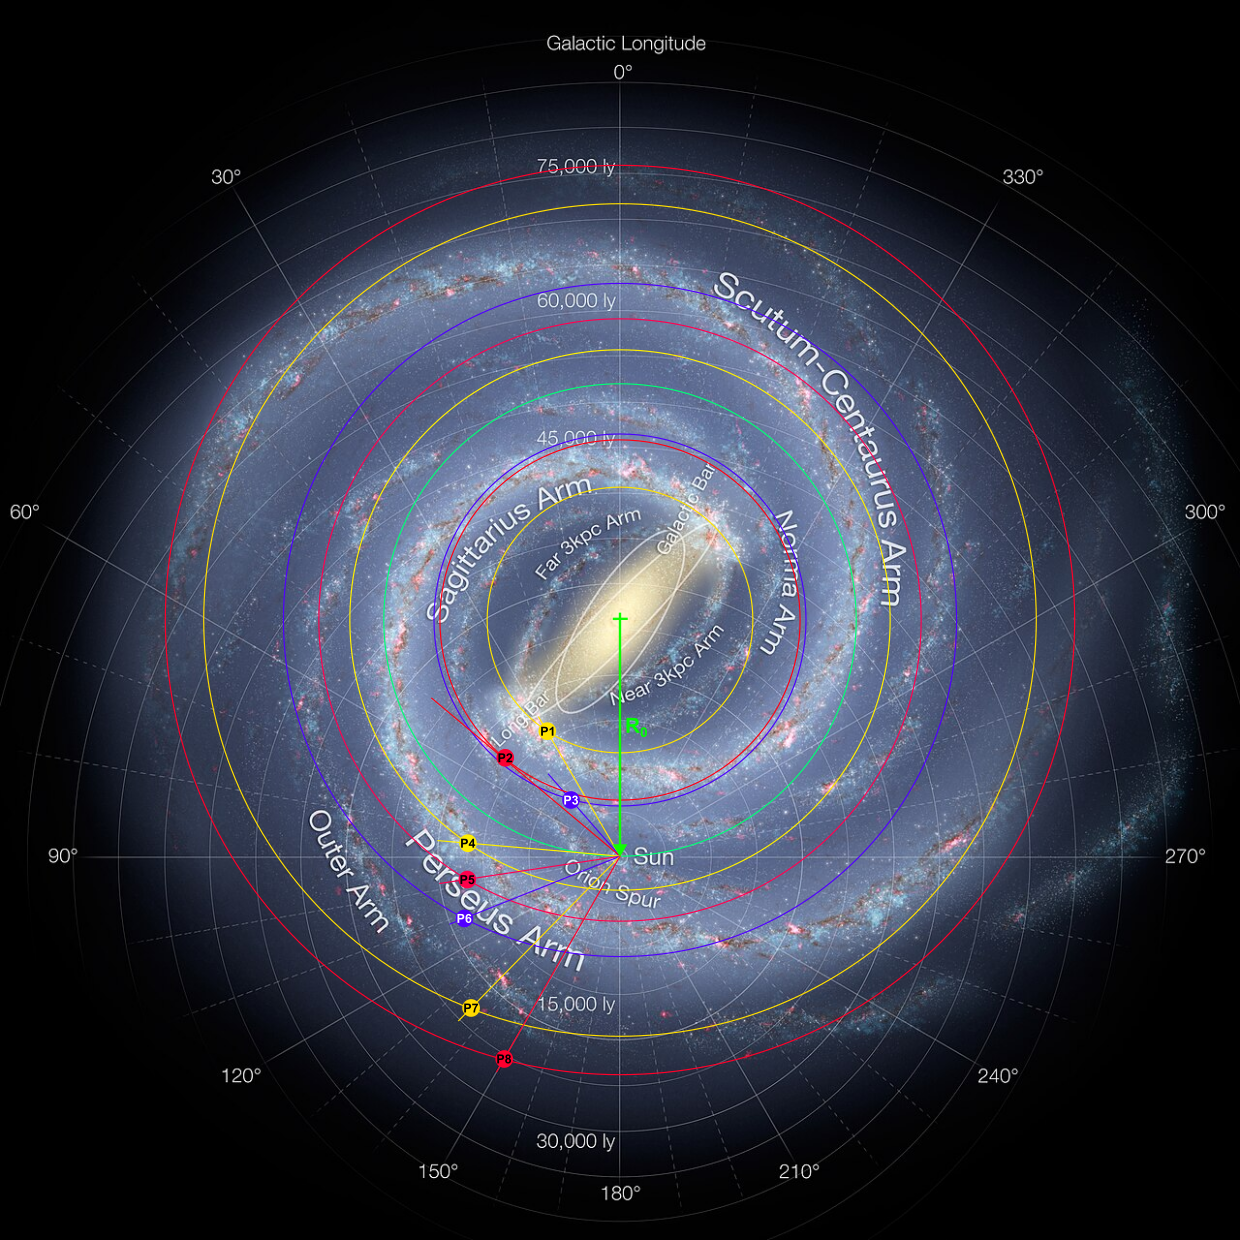
\includegraphics[width=\textwidth]{assets/MW_ROI_spots.png}
    \caption{Bla, Referenz XXXXXX}
    \label{fig:mw_roi_spots}
\end{figure}

We can see that most points are located in spiral arms with mutch higher concentrations of hydrogen. We suppose the sources for the hot spots in the spectrum plot are:
\begin{itemize}
	\item P1: Inner end of Scutum-Centaurs arm, at the near end of the long bar.
	\item P2, P3: Sources located in the Saggitarius arm
	\item P4, P5, P6: Sources located in the Perseus arm
	\item P7, P8: Not sure, maybe locations in the outer arm.
\end{itemize}

TODO (maybe) modelling Perseus arm and show expected red-shift.... 